\pdfminorversion=4
\documentclass[aspectratio=169]{beamer}

\mode<presentation>
{
  \usetheme{default}
  \usecolortheme{default}
  \usefonttheme{default}
  \setbeamertemplate{navigation symbols}{}
  \setbeamertemplate{caption}[numbered]
  \setbeamertemplate{footline}[frame number]  % or "page number"
  \setbeamercolor{frametitle}{fg=white}
  \setbeamercolor{footline}{fg=black}
} 

\usepackage[english]{babel}
\usepackage[utf8x]{inputenc}
\usepackage{tikz}
\usepackage{courier}
\usepackage{array}
\usepackage{bold-extra}
\usepackage{minted}
\usepackage[thicklines]{cancel}
\usepackage{fancyvrb}

\xdefinecolor{dianablue}{rgb}{0.18,0.24,0.31}
\xdefinecolor{darkblue}{rgb}{0.1,0.1,0.7}
\xdefinecolor{darkgreen}{rgb}{0,0.5,0}
\xdefinecolor{darkgrey}{rgb}{0.35,0.35,0.35}
\xdefinecolor{darkorange}{rgb}{0.8,0.5,0}
\xdefinecolor{darkred}{rgb}{0.7,0,0}
\definecolor{darkgreen}{rgb}{0,0.6,0}
\definecolor{mauve}{rgb}{0.58,0,0.82}

\title[2019-10-17-pyhep-awkward]{Uproot and Awkward-Array in the Year of Python}
\author{Jim Pivarski}
\institute{Princeton University -- IRIS-HEP}
\date{October 17, 2019}

\usetikzlibrary{shapes.callouts}

\begin{document}

\logo{\pgfputat{\pgfxy(0.11, 7.4)}{\pgfbox[right,base]{\tikz{\filldraw[fill=dianablue, draw=none] (0 cm, 0 cm) rectangle (50 cm, 1 cm);}\mbox{\hspace{-8 cm}\includegraphics[height=1 cm]{princeton-logo-long.png}\hspace{0.1 cm}\raisebox{0.1 cm}{\includegraphics[height=0.8 cm]{iris-hep-logo-long.png}}\hspace{0.1 cm}}}}}

\begin{frame}
  \titlepage
\end{frame}

\logo{\pgfputat{\pgfxy(0.11, 7.4)}{\pgfbox[right,base]{\tikz{\filldraw[fill=dianablue, draw=none] (0 cm, 0 cm) rectangle (50 cm, 1 cm);}\mbox{\hspace{-8 cm}\includegraphics[height=1 cm]{princeton-logo.png}\hspace{0.1 cm}\raisebox{0.1 cm}{\includegraphics[height=0.8 cm]{iris-hep-logo.png}}\hspace{0.1 cm}}}}}

% Uncomment these lines for an automatically generated outline.
%\begin{frame}{Outline}
%  \tableofcontents
%\end{frame}

% START START START START START START START START START START START START START

\begin{frame}{}
\huge
\vspace{1 cm}
\begin{center}
\textcolor{darkblue}{Year of Python?}
\end{center}
\end{frame}

\begin{frame}{On Scientific Linux, uproot/awkward is installed as often as Pandas}
\vspace{0.5 cm}
\begin{columns}
\column{1.2\linewidth}
\includegraphics[width=\linewidth]{pip-scilinux-uproot.pdf}
\end{columns}
\end{frame}

\begin{frame}{And so is Coffea\ldots}
\vspace{0.5 cm}
\begin{columns}
\column{1.2\linewidth}
\includegraphics[width=\linewidth]{pip-scilinux-uproot-iminuit.pdf}
\end{columns}
\end{frame}

\begin{frame}{\ldots more so than deep learning libraries (TensorFlow and Torch)}
\vspace{0.5 cm}
\begin{columns}
\column{1.2\linewidth}
\includegraphics[width=\linewidth]{pip-scilinux-ml.pdf}
\end{columns}
\end{frame}

\begin{frame}{But take a step back and look in linear scale!}
\vspace{0.5 cm}
\begin{columns}
\column{1.2\linewidth}
\includegraphics[width=\linewidth]{pip-scilinux-linear.pdf}
\end{columns}
\end{frame}

\begin{frame}{The bigger news is that more physicists are using Python {\it this year}}
\vspace{0.5 cm}
\begin{columns}
\column{1.2\linewidth}
\includegraphics[width=\linewidth]{pip-scilinux-everything.pdf}
\end{columns}
\end{frame}

\begin{frame}{Another way to see Python usage among physicists: GitHub repos}
\begin{columns}
\column{1.2\linewidth}
\only<1>{\includegraphics[width=\linewidth]{github-linear.pdf}}\only<2>{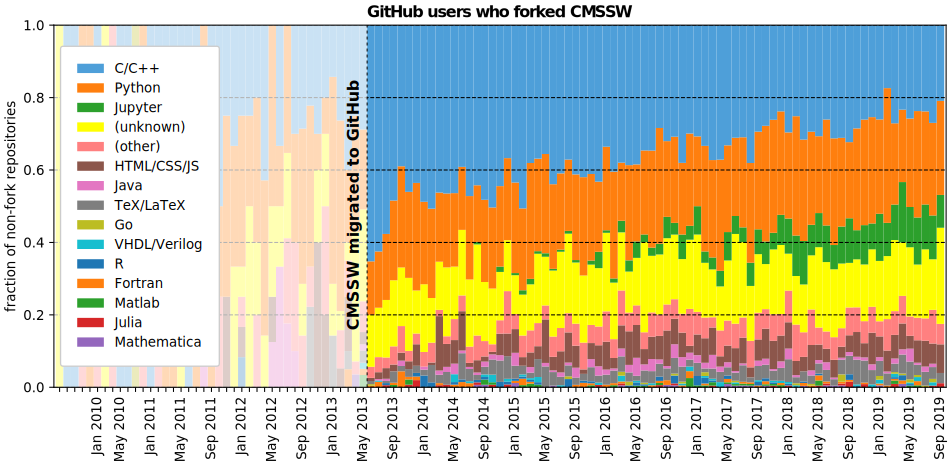
\includegraphics[width=\linewidth]{github-fraction.pdf}}\only<3>{\includegraphics[width=\linewidth]{github-simplefraction.pdf}}
\end{columns}
\end{frame}

\begin{frame}{In a sense, this is the third phase transition for our field}
\vspace{0.5 cm}
\begin{columns}
\column{1.1\linewidth}
\includegraphics[width=\linewidth]{programming-languages.pdf}
\end{columns}
\end{frame}

\begin{frame}{Uproot/Awkward maintainance is pretty much constant}
\Large
\vspace{0.75 cm}
\begin{columns}
\column{0.36\linewidth}
\includegraphics[width=\linewidth]{uproot-issues.pdf}

\column{0.72\linewidth}
\only<1>{\includegraphics[width=0.5\linewidth]{uproot-users.pdf}\hfill\includegraphics[width=0.5\linewidth]{uproot-comments.pdf}}\only<2->{\hfill\includegraphics[width=0.45\linewidth]{uproot-response-time.pdf}\hfill\includegraphics[width=0.45\linewidth]{uproot-response-time-linear.pdf}}
\end{columns}

\vspace{0.25 cm}
\begin{center}
\uncover<3->{The problem with GitHub issues is that once closed, they disappear.}
\end{center}
\end{frame}

\begin{frame}{Let's use StackOverflow (like most non-HEP software communities)}
\begin{center}
\includegraphics[width=0.88\linewidth]{uproot-stackoverflow.png}
\end{center}
\end{frame}

\begin{frame}{No, seriously, do it now.}
\vspace{0.15 cm}
\begin{columns}
\column{1.2\linewidth}
\includegraphics[width=\linewidth]{stackoverflow-signup.png}
\end{columns}
\end{frame}

\begin{frame}{}
\huge
\vspace{1 cm}
\begin{center}
\textcolor{darkblue}{Future of Uproot and Awkward}
\end{center}
\end{frame}

\begin{frame}{Future of uproot: maintenance}
\Large
\vspace{0.35 cm}
\begin{itemize}\setlength{\itemsep}{0.25 cm}
\item<1-> TTree-writing was the last {\it major} feature planned.
\item<2-> Bugs will be fixed.
\item<3-> Uproot will keep ahead of changes in ROOT I/O.

\vspace{0.05 cm}
\textcolor{gray}{\normalsize (Only one change in ROOT I/O in uproot's two-year existence: \mintinline{c++}{TIOFeatures}.)}

\item<4-> ROOT's future \mintinline{c++}{RNtuple} can probably be handled with semi-independent code, as uproot-methods is now.
\item<5-> ``Uproot 4.0'' will be a transition to Awkward 1.0.
\end{itemize}

\normalsize
\vspace{0.25 cm}
\uncover<6->{\textcolor{gray}{(Apart from TTree-writing, uproot has been in maintenance mode for a year already.)}}
\end{frame}

\begin{frame}{Future of awkward: ``consolidation''}
\Large
\vspace{0.35 cm}
\begin{itemize}\setlength{\itemsep}{0.25 cm}
\item<1-> Awkward has been tested ``in the wild'' for a year now.
\item<2-> Pure Numpy implementation does some complex (clever!) things to perform jagged operations: no \mintinline{python}{for} loops allowed.

\vspace{0.1 cm}
\begin{itemize}\setlength{\itemsep}{0.2 cm}
\item<3-> \large There are limits to cleverness: many edge cases not handled.
\item<4-> \large Most frequent bugs are due to Numpy usage (e.g.\ \mintinline{python}{numpy.max([])}).
\item<5-> \large Desire to use awkward-arrays in Numba, on GPUs, and in C++ library interfaces leads to duplication; hard to synchronize implementations.
\end{itemize}

\item<6-> Feedback from users revealed some design mistakes.

\vspace{0.1 cm}
\begin{itemize}\setlength{\itemsep}{0.2 cm}
\item<7-> \large \mintinline{python}{a.cross(b)} versus \mintinline{python}{awkward.cross(a, b)}
\item<8-> \large User-visible \mintinline{python}{JaggedArray} versus \mintinline{python}{ChunkedArray(JaggedArray)}
\end{itemize}
\end{itemize}
\end{frame}

\begin{frame}{Rewrite/redesign in C and C++}
\large
\vspace{0.5 cm}
\begin{columns}
\column{0.5\linewidth}
\vspace{-0.2 cm}

\textcolor{darkblue}{Layer 1:} Python user interface: a single \mintinline{python}{awkward.Array} class.
\vspace{\baselineskip}

\vspace{0.18 cm}
\textcolor{darkblue}{Layer 2:} Structure classes, ``layout''

(such as \mintinline{python}{JaggedArray}/\mintinline{python}{Table}).
\vspace{\baselineskip}

\vspace{0.18 cm}
\textcolor{darkblue}{Layer 3:} Memory management, array allocation and ownership; reference counting.
\vspace{\baselineskip}

\vspace{0.18 cm}
\textcolor{darkblue}{Layer 4:} Implementations, where we write \mintinline{python}{for} loops. The only layer that needs to be optimized.

\column{0.5\linewidth}
\includegraphics[width=\linewidth]{awkward-1-0-layers.pdf}
\end{columns}
\end{frame}

\begin{frame}[fragile]{Example of what layer 4 looks like}
\tiny
\vspace{0.05 cm}
\begin{columns}
\column{1.1\linewidth}
\begin{minted}{c++}
extern "C" {
  Error awkward_listarray32_getitem_next_at_64(int64_t* tocarry, const int32_t* fromstarts, const int32_t* fromstops,
                                               int64_t lenstarts, int64_t startsoffset, int64_t stopsoffset, int64_t at);
  Error awkward_listarray64_getitem_next_at_64(int64_t* tocarry, const int64_t* fromstarts, const int64_t* fromstops,
                                               int64_t lenstarts, int64_t startsoffset, int64_t stopsoffset, int64_t at);
}

template <typename C, typename T>
Error awkward_listarray_getitem_next_at(T* tocarry, const C* fromstarts, const C* fromstops, int64_t lenstarts,
                                        int64_t startsoffset, int64_t stopsoffset, int64_t at) {
  for (int64_t i = 0;  i < lenstarts;  i++) {
    int64_t length = fromstops[stopsoffset + i] - fromstarts[startsoffset + i];
    int64_t regular_at = at;
    if (regular_at < 0) {
      regular_at += length;
    }
    if (!(0 <= regular_at  &&  regular_at < length)) {
      return "index out of range";
    }
    tocarry[i] = fromstarts[startsoffset + i] + regular_at;
  }
  return kNoError;
}
Error awkward_listarray32_getitem_next_at_64(int64_t* tocarry, const int32_t* fromstarts, const int32_t* fromstops,
                                             int64_t lenstarts, int64_t startsoffset, int64_t stopsoffset, int64_t at) {
  return awkward_listarray_getitem_next_at<int32_t, int64_t>(tocarry, fromstarts, fromstops, lenstarts,
                                                             startsoffset, stopsoffset, at);
}
Error awkward_listarray64_getitem_next_at_64(int64_t* tocarry, const int64_t* fromstarts, const int64_t* fromstops,
                                             int64_t lenstarts, int64_t startsoffset, int64_t stopsoffset, int64_t at) {
  return awkward_listarray_getitem_next_at<int64_t, int64_t>(tocarry, fromstarts, fromstops, lenstarts,
                                                             startsoffset, stopsoffset, at);
}
\end{minted}
\end{columns}
\end{frame}

\begin{frame}[fragile]{Example of what layer 3 looks like (C++)}
\tiny
\vspace{0.05 cm}
\begin{columns}
\column{1.1\linewidth}
\begin{minted}{c++}
  template <>
  const std::shared_ptr<Content> ListArrayOf<int32_t>::getitem_next(const std::shared_ptr<SliceItem> head,
                                                                    const Slice& tail, const Index64& advanced) const {
    int64_t lenstarts = starts_.length();
    if (stops_.length() < lenstarts) {
      throw std::invalid_argument("len(stops) < len(starts)");
    }

    if (head.get() == nullptr) {
      return shallow_copy();
    }

    else if (SliceAt* at = dynamic_cast<SliceAt*>(head.get())) {
      assert(advanced.length() == 0);
      std::shared_ptr<SliceItem> nexthead = tail.head();
      Slice nexttail = tail.tail();
      Index64 nextcarry(lenstarts);
      Error err = awkward_listarray32_getitem_next_at_64(
        nextcarry.ptr().get(),
        starts_.ptr().get(),
        stops_.ptr().get(),
        lenstarts,
        starts_.offset(),
        stops_.offset(),
        at->at());
      std::shared_ptr<Content> nextcontent = content_.get()->carry(nextcarry);
      return nextcontent.get()->getitem_next(nexthead, nexttail, advanced);
    }

    else if (SliceRange* range = dynamic_cast<SliceRange*>(head.get())) {
      ...
\end{minted}
\end{columns}
\end{frame}

\begin{frame}[fragile]{Example of what layer 3 looks like (Numba)}
\tiny
\vspace{0.05 cm}
\begin{columns}
\column{1.1\linewidth}
\begin{minted}{python}
@numba.extending.register_model(ListOffsetArrayType)
class ListOffsetArrayModel(numba.datamodel.models.StructModel):
    def __init__(self, dmm, fe_type):
        members = [("offsets", fe_type.offsetstpe),
                   ("content", fe_type.contenttpe)]
        if fe_type.idtpe != numba.none:
            members.append(("id", fe_type.idtpe))
        super(ListOffsetArrayModel, self).__init__(dmm, fe_type, members)

@numba.extending.lower_builtin(operator.getitem, ListOffsetArrayType, numba.types.slice2_type)
def lower_getitem_slice(context, builder, sig, args):
    rettpe, (tpe, wheretpe) = sig.return_type, sig.args
    val, whereval = args

    proxyin = numba.cgutils.create_struct_proxy(tpe)(context, builder, value=val)

    proxyslicein = numba.cgutils.create_struct_proxy(wheretpe)(context, builder, value=whereval)
    proxysliceout = numba.cgutils.create_struct_proxy(numba.types.slice2_type)(context, builder)
    proxysliceout.start = proxyslicein.start
    proxysliceout.stop = builder.add(proxyslicein.stop, context.get_constant(numba.intp, 1))
    proxysliceout.step = context.get_constant(numba.intp, 1)

    proxyout = numba.cgutils.create_struct_proxy(tpe)(context, builder)
    proxyout.offsets = numba.targets.arrayobj.getitem_arraynd_intp(context, builder,
                                                                   tpe.offsetstpe(tpe.offsetstpe, numba.types.slice2_type),
                                                                   (proxyin.offsets, proxysliceout._getvalue()))
    proxyout.content = proxyin.content
    out = proxyout._getvalue()
    if context.enable_nrt:
        context.nrt.incref(builder, rettpe, out)
    return out
\end{minted}
\end{columns}
\end{frame}

\begin{frame}[fragile]{Example of what tests of layer 2 look like}
\tiny
\vspace{0.05 cm}
\begin{columns}
\column{1.1\linewidth}
\begin{minted}{python}
def test_listarray_slice_slice():
    assert awkward1.tolist(array1[2:]) == [[4.4, 5.5], [6.6], [7.7, 8.8, 9.9]]
    assert awkward1.tolist(array1[2:, 1:]) == [[5.5], [], [8.8, 9.9]]
    assert awkward1.tolist(array1[2:,:-1]) == [[4.4], [], [7.7, 8.8]]

def test_listarray_ellipsis():
    if not py27:
        assert awkward1.tolist(array1[Ellipsis, 1:]) == [[2.2, 3.3], [], [5.5], [], [8.8, 9.9]]
        assert awkward1.tolist(array2[Ellipsis, 1:]) == [[[2.2, 3.3], []], [[5.5]], [], [[], [8.8, 9.9]]]

def test_listarray_array_slice():
    assert awkward1.tolist(array2[[0, 0, 1, 1, 1, 0]]) == [[[1.1, 2.2, 3.3], []], [[1.1, 2.2, 3.3], []], [[4.4, 5.5]],
                                                           [[4.4, 5.5]], [[4.4, 5.5]], [[1.1, 2.2, 3.3], []]]
    assert awkward1.tolist(array2[[0, 0, 1, 1, 1, 0], :]) == [[[1.1, 2.2, 3.3], []], [[1.1, 2.2, 3.3], []], [[4.4, 5.5]],
                                                              [[4.4, 5.5]], [[4.4, 5.5]], [[1.1, 2.2, 3.3], []]]
    assert awkward1.tolist(array2[[0, 0, 1, 1, 1, 0], :, 1:]) == [[[2.2, 3.3], []], [[2.2, 3.3], []], [[5.5]], [[5.5]],
                                                                  [[5.5]], [[2.2, 3.3], []]]

def test_listarray_array():
    assert awkward1.tolist(array1[numpy.array([2, 0, 0, 1, -1])]) == [[4.4, 5.5], [1.1, 2.2, 3.3], [1.1, 2.2, 3.3], [],
                                                                      [7.7, 8.8, 9.9]]
    assert awkward1.tolist(array1[numpy.array([2, 0, 0, -1]), numpy.array([1, 1, 0, 0])]) == [5.5, 2.2, 1.1, 7.7]

    assert awkward1.tolist(array1_deep) == [[[0, 0], [1, 10], [2, 20]], [[3, 30], [4, 40], [5, 50]], [[6, 60], [7, 70],
                                                                                                      [8, 80]]]
    s = (numpy.array([2, 0, 0, -1]), numpy.array([1, 1, 0, 0]), numpy.array([0, 1, 0, 1]))
    assert (numpy.array([[[0, 0], [1, 10], [2, 20]], [[3, 30], [4, 40], [5, 50]], [[6, 60], [7, 70], [8, 80]]])[s].tolist()
              == awkward1.tolist(array1_deep[s]))

    s = (numpy.array([2, 0, 0, -1]), numpy.array([1, 1, 0, 0]), slice(1, None))
    assert (numpy.array([[[0, 0], [1, 10], [2, 20]], [[3, 30], [4, 40], [5, 50]], [[6, 60], [7, 70], [8, 80]]])[s].tolist()
              == awkward1.tolist(array1_deep[s]))
\end{minted}
\end{columns}
\end{frame}

\begin{frame}[fragile]{Usable in C++, too (for making interfaces to C++ libraries)}
\tiny
\vspace{0.05 cm}
\begin{columns}
\column{1.1\linewidth}
\begin{minted}{c++}
#include <cassert>

#include "awkward/Identity.h"
#include "awkward/RawArray.h"
#include "awkward/Slice.h"

using namespace awkward;

void slices() {
  RawArrayOf<float> data(Identity::none(), 9);
  *data.borrow(0) = 0.0f;
  *data.borrow(1) = 1.1f;
  *data.borrow(2) = 2.2f;
  *data.borrow(3) = 3.3f;
  *data.borrow(4) = 4.4f;
  *data.borrow(5) = 5.5f;
  *data.borrow(6) = 6.6f;
  *data.borrow(7) = 7.7f;
  *data.borrow(8) = 8.8f;
  *data.borrow(9) = 9.9f;

  Slice at1(std::vector<std::shared_ptr<SliceItem>>({ std::shared_ptr<SliceItem>(new SliceAt(1)) }), true);
  assert(*dynamic_cast<RawArrayOf<float>*>(data.getitem(at1).get())->borrow() == 1.1f);
  Slice at2(std::vector<std::shared_ptr<SliceItem>>({ std::shared_ptr<SliceItem>(new SliceAt(2)) }), true);
  assert(*dynamic_cast<RawArrayOf<float>*>(data.getitem(at2).get())->borrow() == 2.2f);

  Slice range1(std::vector<std::shared_ptr<SliceItem>>({ std::shared_ptr<SliceItem>(new SliceRange(1, 3, Slice::none())) }));
  assert(*dynamic_cast<RawArrayOf<float>*>(data.getitem(range1).get())->borrow(0) == 1.1f);

  Slice range2(std::vector<std::shared_ptr<SliceItem>>({ std::shared_ptr<SliceItem>(new SliceRange(Slice::none(), 4, 1)) }));
  assert(*dynamic_cast<RawArrayOf<float>*>(data.getitem(range2).get())->borrow(0) == 0.0f);
}
\end{minted}
\end{columns}
\end{frame}

\begin{frame}{Timeframe for Awkward 1.0}
\large
\vspace{0.25 cm}
\begin{itemize}\setlength{\itemsep}{0.25 cm}
\item First month (complete):
\begin{itemize}\setlength{\itemsep}{0.1 cm}
\item[\textcolor{darkblue}{$\surd$}] Set up compilation and deployment chain on ManyLinux, MacOS, and Windows.
\item[\textcolor{darkblue}{$\surd$}] Create basic \mintinline{c++}{NumpyArray}/\mintinline{c++}{ListArray} suite and ensure proper reference counting between Python, \mintinline{c++}{std::shared_ptr}, and Numba's NRT.
\item[\textcolor{darkblue}{$\surd$}] Pass through new ``\mintinline{c++}{Identity}'' arrays (Pandas-style index) at every level.
\item[\textcolor{darkblue}{$\surd$}] Access the same layer 4 functions in C++ and Numba.
\end{itemize}

\item Second month (in progress):
\begin{itemize}
\item[\textcolor{darkblue}{$\surd$}] Implement Numpy's \mintinline{python}{__getitem__} in full generality.
\item Implement \mintinline{python}{awkward.fromiter}/\mintinline{python}{append} to grow columnar arrays.
\item Layer 1 \mintinline{python}{awkward.Array} class as a user interface.
\end{itemize}

\item Beyond that,
\begin{itemize}
\item User-defined mix-in methods in layer 1.
\item More array types \mintinline{c++}{RecordArray}, \mintinline{c++}{MaskedArray}, \mintinline{c++}{ChunkedArray}\ldots
\end{itemize}

\item Transition {\normalsize \mintinline{python}{import awkward}} $\to$ {\normalsize \mintinline{python}{import awkward0}}

\hspace{1.1 cm}and {\normalsize \mintinline{python}{import awkward1}} $\to$ {\normalsize \mintinline{python}{import awkward}} in early 2020.
\end{itemize}
\end{frame}

\begin{frame}{}
\huge
\vspace{1 cm}
\begin{center}
\textcolor{darkblue}{BACKUP}
\end{center}
\end{frame}

\begin{frame}{(In general, uproot is 4 orders of magnitude below Pandas)}
\vspace{0.5 cm}
\begin{columns}
\column{1.2\linewidth}
\only<1>{\includegraphics[width=\linewidth]{pip-linux.pdf}}\only<2>{\includegraphics[width=\linewidth]{pip-macos.pdf}}\only<3>{\includegraphics[width=\linewidth]{pip-windows.pdf}}
\end{columns}
\end{frame}

\begin{frame}[fragile]{Analysis of pip download data \only<1-3>{(Google BigQuery)}\only<4>{(GitHub API)}}
\vspace{0.5 cm}
\scriptsize

\textcolor{blue}{\url{https://github.com/jpivarski/2019-10-17-pyhep-awkward/blob/master/analysis.ipynb}}

\vspace{0.25 cm}
\begin{onlyenv}<1>
\begin{minted}{sql}
SELECT
  DATE(timestamp) AS date,
  CASE WHEN country_code = "CH" THEN "CH" WHEN country_code = "US" THEN "US"
       ELSE "other" END AS country,
  file.project AS project,
  REGEXP_REPLACE(file.version, "\\.[0123456789]{1,}$", "") AS version,
  COUNT(*) AS count
FROM `the-psf.pypi.downloads*`
WHERE
  _TABLE_SUFFIX BETWEEN '20160101' AND '20190922'
  AND (file.project = "uproot" OR         file.project = "awkward" OR
       file.project = "iminuit" OR        file.project = "matplotlib" OR
       file.project = "pandas" OR         file.project = "numpy" OR
       file.project = "tensorflow" OR     file.project = "torch" OR
       file.project = "Keras" OR          file.project = "scikit-learn" OR
       file.project = "scipy")
  AND details.distro.name LIKE "%Scientific%" AND details.installer.name = "pip"
GROUP BY project, version, date, country
ORDER BY project, version, date, country
\end{minted}
\vspace{10 cm}
\end{onlyenv}\begin{onlyenv}<2>
\begin{minted}{sql}
SELECT
  DATE(timestamp) AS date,
  details.system.name AS os,
  file.project AS project,
  REGEXP_REPLACE(file.version, "\\.[0123456789]{1,}$", "") AS version,
  COUNT(*) AS count
FROM `the-psf.pypi.downloads*`
WHERE
  _TABLE_SUFFIX BETWEEN '20160101' AND '20190922'
  AND (file.project = "uproot" OR         file.project = "awkward" OR
       file.project = "iminuit" OR        file.project = "matplotlib" OR
       file.project = "pandas" OR         file.project = "numpy" OR
       file.project = "tensorflow" OR     file.project = "torch" OR
       file.project = "Keras" OR          file.project = "scikit-learn" OR
       file.project = "scipy")
  AND details.installer.name = "pip"
GROUP BY project, version, date, os
ORDER BY project, version, date, os
\end{minted}
\vspace{10 cm}
\end{onlyenv}\begin{onlyenv}<3>
\begin{minted}{sql}
SELECT
  DATE(timestamp) AS date,
  CASE WHEN country_code = "CH" THEN "CH" WHEN country_code = "US" THEN "US"
       ELSE "other" END AS country,
  COUNT(*) AS count
FROM `the-psf.pypi.downloads*`
WHERE
  _TABLE_SUFFIX BETWEEN '20160101' AND '20190922'
  AND details.distro.name LIKE "%Scientific%" AND details.installer.name = "pip"
GROUP BY date, country
ORDER BY date, country
\end{minted}
\vspace{10 cm}
\end{onlyenv}\begin{onlyenv}<4>
\begin{minted}{bash}
for x in 1 ... 97; do curl "https://api.github.com/repos/cms-sw/cmssw/forks?page=$x"
  -u 'USERNAME:PASSWORD' > github-cmssw/forks-$x.json; echo $x; done

python -c 'import json, glob; print("\n".join([fork["owner"]["login"] for filename in
  glob.glob("github-cmssw/forks-*.json") for fork in json.load(open(filename))]))'
  > github-cmssw/users.txt

for x in `cat github-cmssw/users.txt`; do curl "https://api.github.com/users/$x/repos
  ?per_page=100" -u 'USERNAME:PASSWORD' > github-cmssw/user-$x.json; echo $x; done

python -c 'import json, glob; print("repo,owner,isfork,created,language"); print("\n"
  .join([",".join(map(str, [repo["name"], repo["owner"]["login"], repo["fork"],
  repo["created_at"], repr(repo["language"])])) for filename in glob.glob("github-cmssw
  /user-*.json") for repo in json.load(open(filename))]))' > github-cmssw.csv

curl "https://api.github.com/repos/scikit-hep/REPOSITORY/issues?state=all&page=PAGENUM
  &per_page=100" >> github-issues-REPOSITORY.json

python -c 'import json; print("number,title,user,state,date_created,date_closed,
  numcomments,ispull"); print("\n".join([",".join([str(x["number"]), json.dumps(
  x["title"]), x["user"]["login"], x["state"], str(x["created_at"]), str(x["closed_at"]),
  str(x["comments"]), str("pull_request" in x)]) for x in json.load(open("github-issues
  -REPOSITORY.json"))]))' > github-issues-REPOSITORY.csv 
\end{minted}
\vspace{10 cm}
\end{onlyenv}
\end{frame}

\begin{frame}{Year of Python, so what do I do? Go back to C++\ldots}
\vspace{0.5 cm}
\begin{columns}
\column{1.1\linewidth}
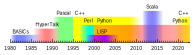
\includegraphics[width=\linewidth]{personal-programming-languages.pdf}
\end{columns}
\end{frame}

\end{document}
